% Generated by scripts/convert_report.py from source/report.md.


\FloatBarrier

\Needspace{6\baselineskip}

\section{HIỆN THỰC HỆ THỐNG}


Chương này trình bày các thành phần chính được hiện thực để xây dựng nền tảng MLOps trên AWS, tập trung vào quản lý hạ tầng, tự động hóa huấn luyện, triển khai dịch vụ và kiểm soát phát hành. Kết quả kiểm chứng và đánh giá hệ thống được trình bày tại Chương 4.


\subsection{Triển khai hạ tầng AWS và Kubernetes}


\subsubsection{Quản lý hạ tầng bằng Terraform}


Hạ tầng được triển khai bằng Terraform, với mã nguồn tổ chức trong thư mục \code{infra/terraform/}. Các tài nguyên được quản lý thông qua ba lớp Bootstrap, Persistent và Platform như đã trình bày ở Chương 2. Việc phân tách này cho phép quản lý vòng đời hạ tầng độc lập với những dữ liệu và artifacts cần được bảo toàn.


Trong quá trình hiện thực, nhóm sử dụng Terraform để cấu hình VPC trên hai Availability Zones, hệ thống mạng public/private subnets, Amazon EKS và các dịch vụ lưu trữ liên quan. Các tài nguyên lưu trữ quan trọng được áp dụng cơ chế mã hóa, versioning và hạn chế xóa ngoài ý muốn. Quá trình triển khai được thực hiện thông qua \code{terraform plan} và \code{terraform apply} để kiểm tra thay đổi trước khi áp dụng lên AWS.


\begin{figure}[!htbp]\centering
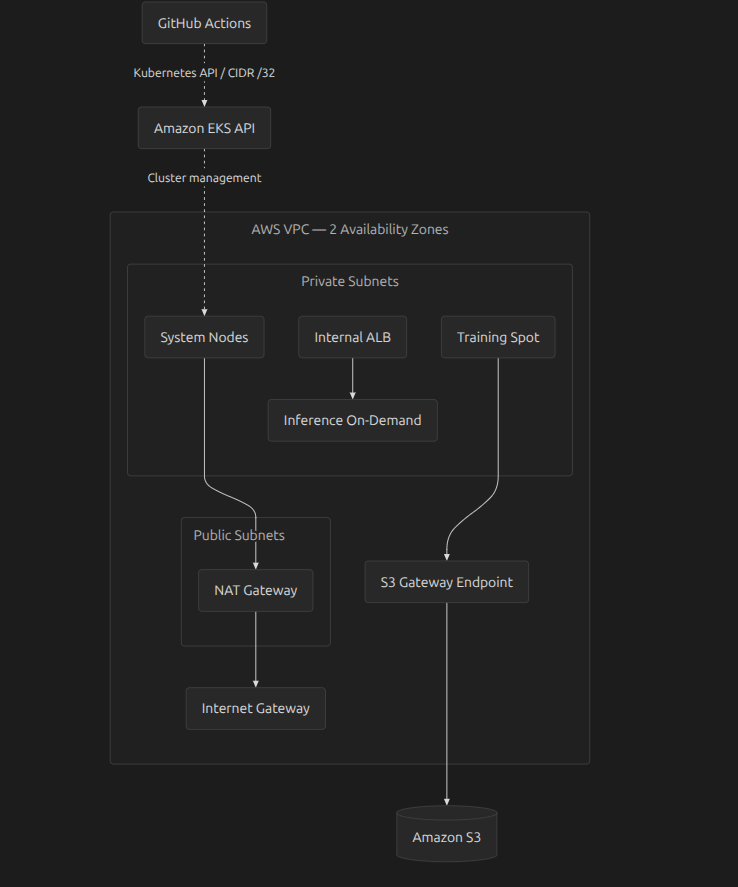
\includegraphics[width=0.86\linewidth,height=0.62\textheight,keepaspectratio]{Pictures/network.png}
\caption{Cấu trúc mạng và các thành phần hạ tầng triển khai trên AWS.}
\label{fig:network}
\end{figure}
\FloatBarrier

\subsubsection{Điều phối tài nguyên và quản lý quyền truy cập}


Amazon EKS được sử dụng để vận hành các thành phần của nền tảng dưới dạng Kubernetes workloads. Nhóm triển khai Managed Node Group \code{system} cho các dịch vụ nền và sử dụng Karpenter để quản lý hai NodePool chuyên biệt:


\begin{itemize}

\item 

\textbf{\code{training-spot}}\textbf{:} Cấp phát Spot Instances cho các Kubernetes Jobs huấn luyện mô hình.


\item 

\textbf{\code{inference-on-demand}}\textbf{:} Sử dụng On-Demand Instances cho dịch vụ FastAPI nhằm hạn chế rủi ro gián đoạn trong quá trình phục vụ.


\end{itemize}

Các workload được phân bổ thông qua node selectors, taints và tolerations. Karpenter hỗ trợ cấp phát tài nguyên khi có nhu cầu và thu hồi các node không còn workload, góp phần hạn chế chi phí vận hành.


Về bảo mật, hệ thống kết hợp AWS IAM, EKS Pod Identity và Kubernetes RBAC để phân quyền truy cập. Các GitHub Actions workflows sử dụng OIDC với IAM Role riêng cho Training và Release, cho phép truy cập AWS bằng credentials tạm thời thay vì lưu trữ access key trực tiếp trong mã nguồn.


\subsection{Pipeline huấn luyện và quản lý mô hình}


\subsubsection{Xây dựng và thực thi Training Pipeline}


Pipeline huấn luyện được hiện thực trong \code{src/training/}, sử dụng LightGBM cho bài toán dự đoán thời lượng chuyến đi taxi. Dữ liệu NYC TLC được xử lý và chia thành các tập training, validation và testing như đã trình bày ở Chương 1, sau đó lưu trữ trên Amazon S3. Logic tạo đặc trưng được tái sử dụng giữa training và inference nhằm bảo đảm tính nhất quán khi triển khai mô hình.


Quy trình huấn luyện trên cloud được thực thi thông qua GitHub Actions workflow \code{train.yml}. Workflow xây dựng container image, đẩy lên Amazon ECR và khởi tạo Kubernetes Training Job trên Spot NodePool của EKS. Job thực hiện huấn luyện, đánh giá mô hình và ghi nhận kết quả vào MLflow, sau đó các tài nguyên tạm được dọn dẹp.


Chất lượng mô hình được đánh giá bằng hai chỉ số \textbf{MAE (Mean Absolute Error)} và \textbf{RMSE (Root Mean Squared Error)}, trong đó MAE được sử dụng làm tiêu chí chính để lựa chọn mô hình. Kết quả đánh giá trên tập validation là cơ sở cho bước kiểm duyệt trước khi đăng ký phiên bản mới.


\subsubsection{Validation Gate và MLflow Model Registry}


Sau huấn luyện, hệ thống sử dụng Validation Gate để kiểm tra chất lượng của mô hình ứng viên so với mô hình tham chiếu. Điều kiện chấp nhận được xác định như sau:


\begin{equation}
\operatorname{MAE}_{\text{candidate}} \leq \operatorname{MAE}_{\text{reference}}\times(1-\delta)
\label{eq:validation-gate}\end{equation}

Trong đó, \(\delta=0{,}01\) tương ứng với yêu cầu cải thiện tối thiểu \textbf{1\% Validation MAE}. Khi đã có mô hình \code{champion}, hệ thống sử dụng phiên bản này làm tham chiếu; trường hợp chưa có phiên bản phù hợp sẽ sử dụng baseline đã xác định.


Nếu candidate không đạt yêu cầu, kết quả thí nghiệm vẫn được lưu trong MLflow Tracking nhưng không tạo phiên bản Model Registry mới. Ngược lại, mô hình đạt điều kiện sẽ được đăng ký và phê duyệt để phục vụ quy trình phát hành.


MLflow sử dụng PostgreSQL để quản lý metadata và Amazon S3 để lưu trữ model artifacts, kèm thông tin định danh nhằm hỗ trợ truy vết phiên bản. Hệ thống cũng hiện thực cơ chế backup/restore cho PostgreSQL để bảo toàn dữ liệu Registry. Alias \code{champion} chỉ được cập nhật sau khi phiên bản mới hoàn tất kiểm chứng triển khai, không thay đổi ngay tại bước huấn luyện.


\subsection{Triển khai dịch vụ suy luận và quy trình CI/CD}


\subsubsection{Xây dựng dịch vụ suy luận với FastAPI}


Dịch vụ suy luận được xây dựng bằng FastAPI, sử dụng mô hình LightGBM đã được phê duyệt trong MLflow Model Registry. Mô hình và các thành phần cần thiết được đóng gói cùng ứng dụng thành Docker image, cho phép xử lý yêu cầu mà không cần truy cập trực tiếp MLflow hoặc S3 trong mỗi lần dự đoán.


Các API chính được triển khai bao gồm:


\begin{table}[!htbp]\centering
\fontsize{12}{15}\selectfont\setstretch{1.05}
\setlength{\tabcolsep}{4pt}\setlength{\arrayrulewidth}{0.4pt}\renewcommand{\arraystretch}{1.2}
\setlength{\ReportTableWidth}{\dimexpr\linewidth-3\arrayrulewidth\relax}
\begin{tabular}{|L{\dimexpr 0.31\ReportTableWidth-2\tabcolsep\relax}|L{\dimexpr 0.69\ReportTableWidth-2\tabcolsep\relax}|}
\hline
\textbf{API} & \textbf{Chức năng} \\
\hline
\code{POST /predict} & Tiếp nhận dữ liệu và trả về kết quả dự đoán. \\\hline
\code{GET /healthz} & Kiểm tra trạng thái hoạt động của ứng dụng. \\\hline
\code{GET /readyz} & Xác nhận dịch vụ sẵn sàng phục vụ. \\\hline
\code{GET /model-info} & Truy xuất thông tin và phiên bản mô hình. \\\hline
\code{GET /metrics} & Cung cấp metrics cho Prometheus. \\\hline
\end{tabular}
\caption{Các API chính của dịch vụ suy luận}\label{tab:09}
\end{table}

Dữ liệu đầu vào được kiểm tra bằng Pydantic và chuyển đổi theo cùng đặc tả đặc trưng đã sử dụng khi huấn luyện. Dịch vụ được triển khai trên EKS với tài nguyên On-Demand để phục vụ các yêu cầu suy luận.


\subsubsection{Tự động hóa CI/CD và triển khai theo GitOps}


Nhóm sử dụng GitHub Actions để tổ chức quy trình tự động hóa thông qua ba workflows:


\begin{table}[!htbp]\centering
\fontsize{12}{15}\selectfont\setstretch{1.05}
\setlength{\tabcolsep}{4pt}\setlength{\arrayrulewidth}{0.4pt}\renewcommand{\arraystretch}{1.2}
\setlength{\ReportTableWidth}{\dimexpr\linewidth-3\arrayrulewidth\relax}
\begin{tabular}{|L{\dimexpr 0.25\ReportTableWidth-2\tabcolsep\relax}|L{\dimexpr 0.75\ReportTableWidth-2\tabcolsep\relax}|}
\hline
\textbf{Workflow} & \textbf{Chức năng} \\
\hline
\code{ci.yml} & Kiểm thử mã nguồn và cấu hình hệ thống. \\\hline
\code{train.yml} & Huấn luyện mô hình trên EKS và thực hiện Validation Gate. \\\hline
\code{release.yml} & Đóng gói, triển khai và xác minh phiên bản mô hình được phê duyệt. \\\hline
\end{tabular}
\caption{Các workflow GitHub Actions}\label{tab:10}
\end{table}

Khi có thay đổi phù hợp trên nhánh \code{main}, hệ thống thực hiện CI và xác định nhu cầu huấn luyện dựa trên thay đổi của mã nguồn. Training workflow chỉ chuyển tiếp sang Release khi mô hình vượt qua Validation Gate, đồng thời sử dụng checkpoint để hạn chế xử lý trùng lặp.


Trong quá trình phát hành, mô hình được đóng gói thành Docker image và lưu trữ trên Amazon ECR với định danh digest bất biến. Release workflow cập nhật image digest trong GitOps manifests, sau đó Argo CD đồng bộ cấu hình mới lên Kubernetes.


Phiên bản mới tiếp tục được kiểm chứng thông qua Canary Deployment trước khi chính thức thay thế phiên bản đang phục vụ. Cách tổ chức này bảo đảm việc kiểm duyệt mô hình và quyết định phát hành được thực hiện độc lập.


\subsection{Triển khai Canary, giám sát và tự động mở rộng}


\subsubsection{Canary Deployment và cơ chế khôi phục}


Hệ thống sử dụng Argo Rollouts kết hợp AWS Application Load Balancer để thực hiện triển khai Canary. Phiên bản ứng viên được kiểm tra bằng Smoke Test trước khi tiếp nhận lưu lượng theo các mức \textbf{10\% và 50\%}, với thời gian quan sát hai phút tại mỗi giai đoạn.


Trong quá trình triển khai, Argo Rollouts sử dụng Prometheus để đánh giá các tiêu chí được cấu hình trong \code{AnalysisTemplate}:


\begin{table}[!htbp]\centering
\fontsize{12}{15}\selectfont\setstretch{1.05}
\setlength{\tabcolsep}{4pt}\setlength{\arrayrulewidth}{0.4pt}\renewcommand{\arraystretch}{1.2}
\setlength{\ReportTableWidth}{\dimexpr\linewidth-3\arrayrulewidth\relax}
\begin{tabular}{|L{\dimexpr 0.42\ReportTableWidth-2\tabcolsep\relax}|L{\dimexpr 0.58\ReportTableWidth-2\tabcolsep\relax}|}
\hline
\textbf{Tiêu chí} & \textbf{Điều kiện chấp nhận} \\
\hline
Tỷ lệ HTTP 5xx của Canary & Nhỏ hơn 1\%. \\\hline
Độ trễ P95 của Canary & Nhỏ hơn 500 ms. \\\hline
P95 so với Stable & Nhỏ hơn \code{1,5 × P95 Stable + 50 ms}. \\\hline
Tốc độ yêu cầu đến Canary & Tối thiểu 0,2 request/giây. \\\hline
\end{tabular}
\caption{Các điều kiện chấp nhận Canary}\label{tab:12}
\end{table}

Để cung cấp lưu lượng đánh giá trong môi trường thực nghiệm, Release workflow sử dụng Kubernetes Job chạy k6 với mức tải cấu hình 40 RPS.


Khi các điều kiện được đáp ứng, phiên bản mới được Promotion và cập nhật alias \code{champion} sau khi xác minh trạng thái phục vụ. Nếu Canary bị từ chối, Argo Rollouts thực hiện Abort để khôi phục lưu lượng về Stable; Release workflow tiếp tục hoàn tác thay đổi GitOps bằng cơ chế guarded Git revert.


Cơ chế khôi phục được áp dụng cho các trường hợp Canary bị từ chối theo điều kiện kiểm duyệt đã xác định, không mặc định bao phủ mọi tình huống lỗi trong quá trình phát hành.


\subsubsection{Giám sát vận hành và tự động mở rộng}


Hệ thống sử dụng Prometheus để thu thập các chỉ số vận hành từ FastAPI, bao gồm request rate, HTTP error rate và latency. Grafana được sử dụng để trực quan hóa metrics, phục vụ việc theo dõi tình trạng hệ thống và đánh giá các thử nghiệm.


Khả năng tự động mở rộng được hiện thực thông qua Horizontal Pod Autoscaler (HPA), với đối tượng điều chỉnh là \code{inference-api} Rollout. HPA được cấu hình từ \textbf{1 đến 3 replica}, sử dụng ngưỡng CPU utilization mục tiêu \textbf{60\%} và thời gian ổn định khi giảm replica là \textbf{300 giây}.


HPA điều chỉnh số lượng Pod theo mức sử dụng CPU, trong khi Karpenter đảm nhiệm việc cấp phát tài nguyên node khi cần thiết. Các cơ chế này được tích hợp vào hệ thống serving để hỗ trợ điều chỉnh năng lực phục vụ theo tải.

